%%%%%%%%%%%%%%%%%%%%%%%%%%%%%%%%%%%%%%%%%%%%%%%%%%%%%%%%%%%%%%%%%%%%%%%%%%%%%%%

\documentclass[12pt,twocolumn,tighten]{aastex62}
%\documentclass[12pt,twocolumn,tighten,trackchanges]{aastex62}
\usepackage{amsmath,amstext,amssymb}
\usepackage[T1]{fontenc}
\usepackage{apjfonts}
\usepackage[figure,figure*]{hypcap}
\usepackage{graphics,graphicx}
\usepackage{hyperref}
\usepackage{natbib}

\renewcommand*{\sectionautorefname}{Section} %for \autoref
\renewcommand*{\subsectionautorefname}{Section} %for \autoref

%% Reintroduced the \received and \accepted commands from AASTeX v5.2.
%% Add "Submitted to " argument.
\received{\today}
\revised{---}
\accepted{---}
\submitjournal{AAS journals.}
\shorttitle{Against PTFO$\,$8-8695b}

\begin{document}

\defcitealias{bouma_wasp4b_2019}{B19}

\title{Against the Planetary Interpretation of PTFO$\,$8-8695b}

\correspondingauthor{L. G. Bouma}
\email{luke@astro.princeton.edu}

%
% key authors:
%
\author[0000-0002-0514-5538]{L. G. Bouma}
\affiliation{ Department of Astrophysical Sciences, Princeton
University, 4 Ivy Lane, Princeton, NJ 08540, USA}
%
\author[0000-0002-4265-047X]{J. N. Winn}
\affiliation{ Department of Astrophysical Sciences, Princeton
University, 4 Ivy Lane, Princeton, NJ 08540, USA}

%
% contributing authors: alphabetical
%
% \author[0000-0001-8638-0320]{A. W. Howard}
% \affiliation{Cahill Center for Astrophysics, California Institute of
% Technology, Pasadena, CA 91125, USA}
% %
% \author[0000-0002-2532-2853]{S. B. Howell}
% \affiliation{NASA Ames Research Center, Moffett Field, CA 94035, USA}
% %
% \author[0000-0002-0531-1073]{H. Isaacson}
% \affiliation{Astronomy Department, University of California, Berkeley,
% CA 94720, USA}
% %
% \author{H. Knutson}
% \affiliation{Division of Geological and Planetary Sciences, California
% Institute of Technology, Pasadena, CA 91125, USA}
% %
% \author[0000-0001-7233-7508]{R. A. Matson}
% \affiliation{U.S. Naval Observatory, Washington, DC 20392, USA}
% %

\begin{abstract}
  PTFO$\,$8-8695b could be the youngest, shortest-period 
  hot Jupiter known.  However it has not been shown to be a planet.
  TESS recently observed PTFO$\,$8-8695 for one month.
  The TESS light-curve shows that the dominant variability in this
  system is a sinusoidal modulation with a ``long'' period $P_{\rm
  \ell}$
  of 11.96 hours, likely caused by stellar rotation.
  Also present is a complex signal, previously identified as the
  planet candidate, that repeats with a ``short'' period $P_{\rm s}$ of
  10.74 hours.
  The ``long'' and ``short'' signals show the expected beat every 4.48
  days.
  There is a dip in the complex, short-period signal.
  However ground-based photometry from the past decade shows that the
  orbital phase of the dip seems to have instantaneously jumped, at
  least once, and maybe twice.
  The TESS epoch of the dip is consistent with recent observations by
  Tanimoto et al., and differs from the discovery epoch by 5.14 hours.
  Planets do not ``jump'' in orbital phase.
  PTFO$\,$8-8695 therefore seems broadly consistent with the
  ``transient dipping'' phenomenology observed in many young M dwarfs,
  and seems unlikely to be a planet.
\end{abstract}

%TODO
\keywords{}

%%%%%%%%%%%%%%%%%%%%%%%%%%%%%%%%%%%%%%%%%%%%%%%%%%%%%%%%%%%%%%%%%%%%%%%%%%%%%%%

\section{Introduction}
If it were a planet, PTFO$\,$8-8695b would be exceptional.
A transiting hot Jupiter, orbiting a $\approx$3$\,$Myr old M dwarf
in ORION would make it the youngest hot Jupiter known.
Its orbital period of only 12 HOURS would also make it the shortest
period hot Jupiter known.

% Section~\ref{sec:observations} of this paper presents all of the
% available transit data as well as the new radial velocity and speckle
% imaging observations.  Section~\ref{sec:analysis} describes our
% analysis of the data, and our interpretation that WASP-4 is being
% pulled around by a brown dwarf or low-mass star.
% Section~\ref{sec:discussion} places this result within the context of
% orbital decay searches, and points out that line-of-sight
% accelerations will be a relatively common type of ``false positive.''
% Section~\ref{sec:conclusions} offers concluding remarks.

\section{Observations}
\label{sec:observations}


\section{Analysis}
\label{sec:analysis}

\begin{figure*}[t]
	\begin{center}
		\leavevmode
		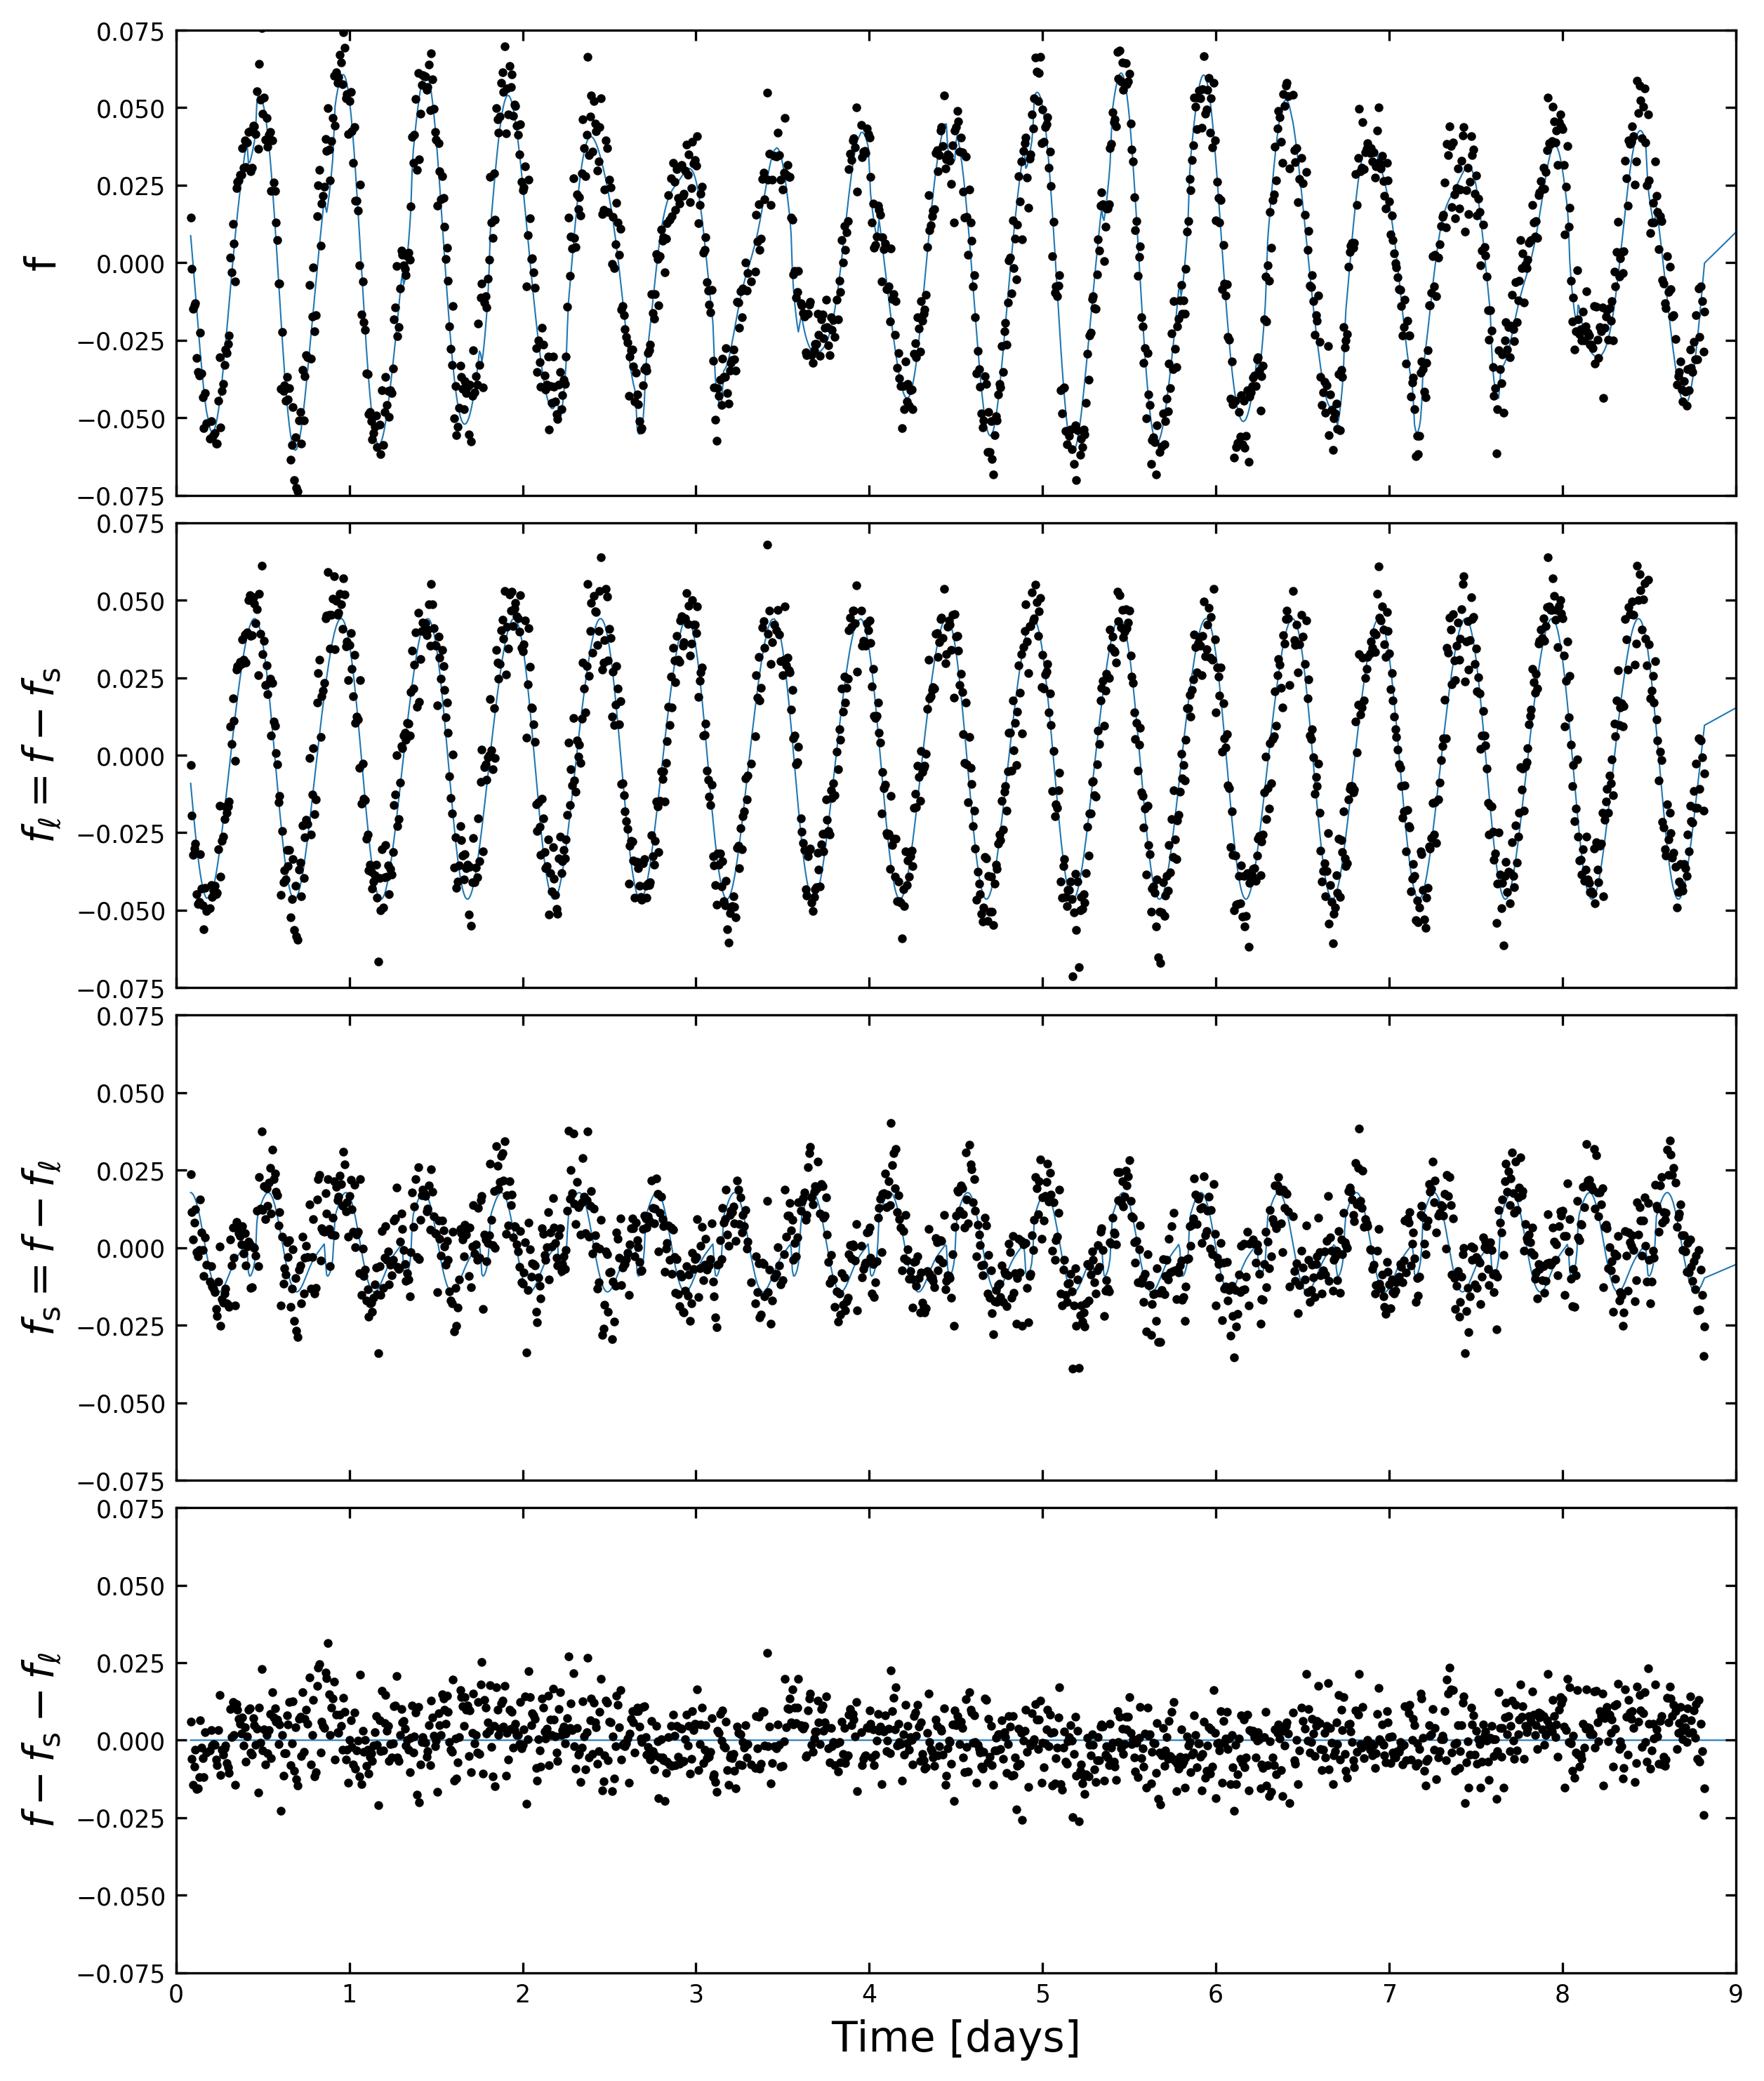
\includegraphics[width=0.98\textwidth]{f1.png}
	\end{center}
	\vspace{-0.7cm}
	\caption{ {\bf TESS light-curve of PTFO 8-8695 (Sector 6, Orbit 1).}
	{\it Top}: ``Raw'' \texttt{PDCSAP} mean-subtracted relative flux versus time. The beat period of 4.48 days is visible by eye.
	The model plotted underneath the data includes 2 harmonics at the long
	period $P_{\rm \ell}$, plus 2 harmonics and a transit at the short period $P_{\rm s}$.
	{\it Upper middle}: Long-period signal, equal to the raw signal minus the short-period signal.
	{\it Lower middle}: Short-period signal, equal to the raw signal minus the long-period signal.
	{\it Bottom}: residual.
	The data are binned from 2 to 10 minute cadence as a convenience for plotting and fitting.
		\label{fig:splitsignal}
	}
\end{figure*}

\begin{figure*}[t]
	\begin{center}
		\leavevmode
		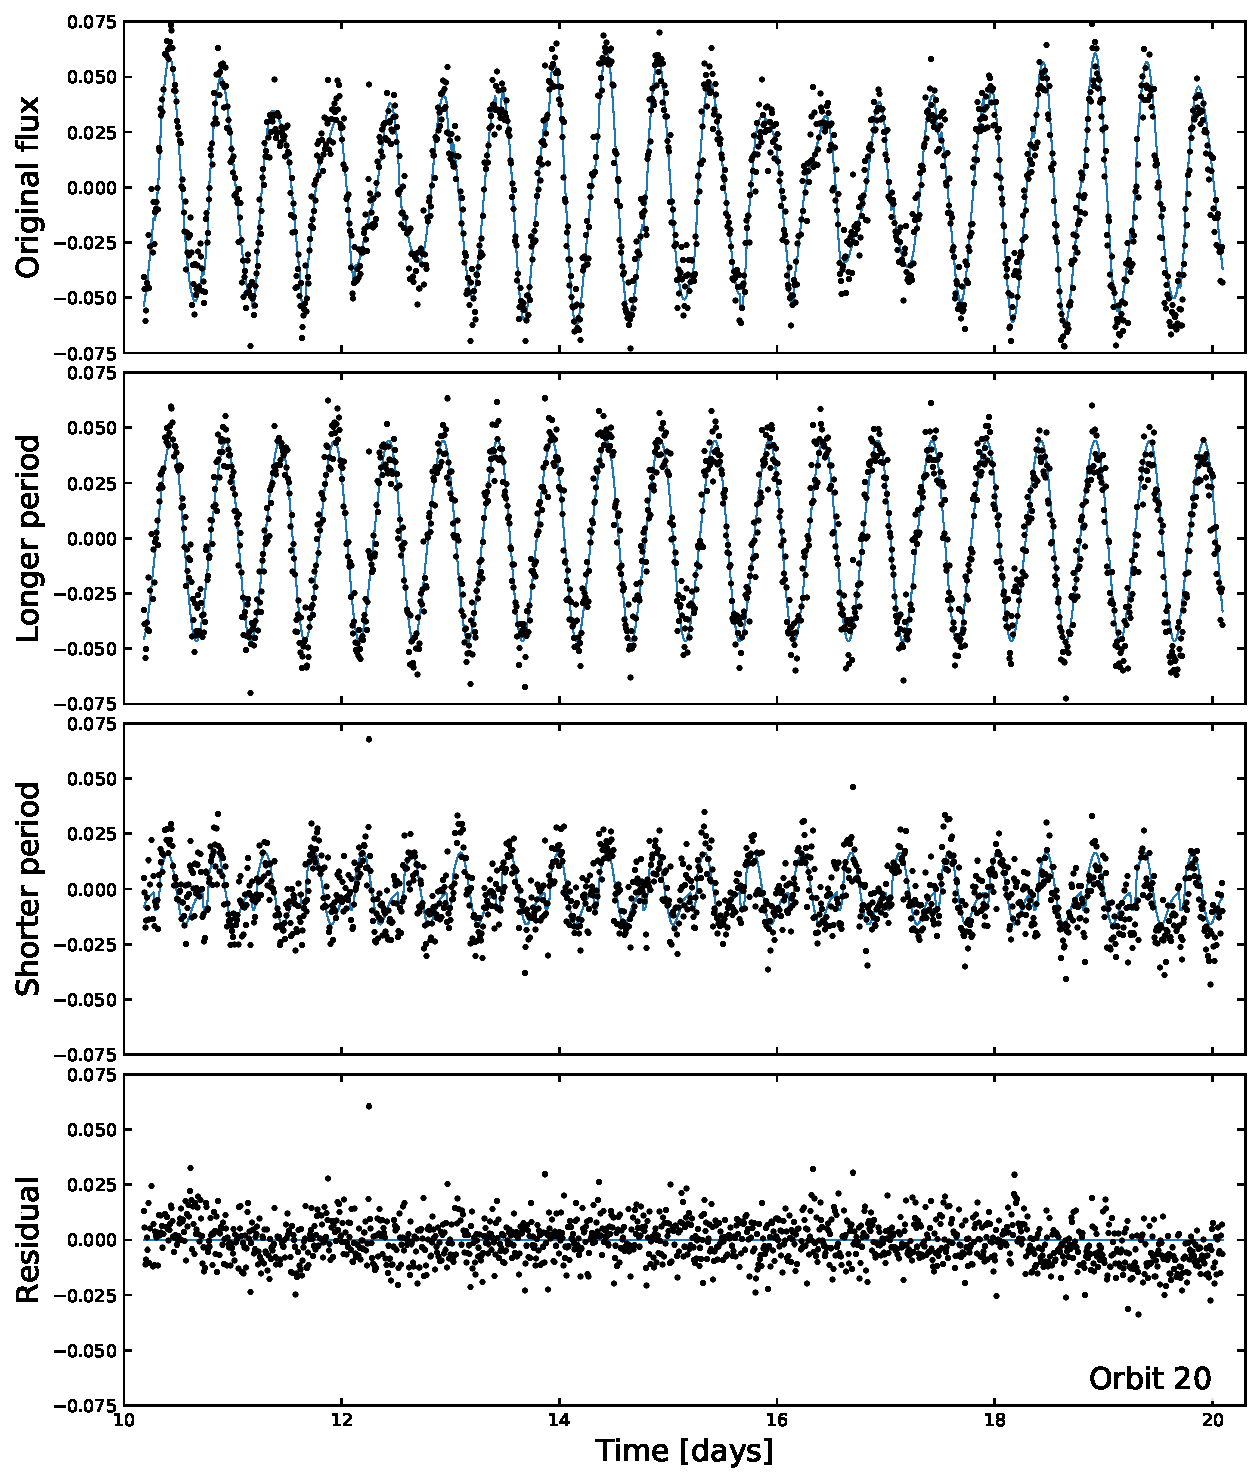
\includegraphics[width=0.95\textwidth]{f2.pdf}
	\end{center}
	\vspace{-0.7cm}
	\caption{ {\bf Phase-folded long and short-period signals.}
	{\it Top}: Long-period signal, as in Figure~\ref{fig:splitsignal}.
	{\it Bottom}: Short-period signal. The reference phase is set to the ``planetary'' dip.
	Gray points are the 10 minute cadence \texttt{PDCSAP} flux.
	Black points are binned to 100 points per period.
	\label{fig:phasefold}
	}
\end{figure*}


\begin{figure}[t]
	\begin{center}
		\leavevmode
		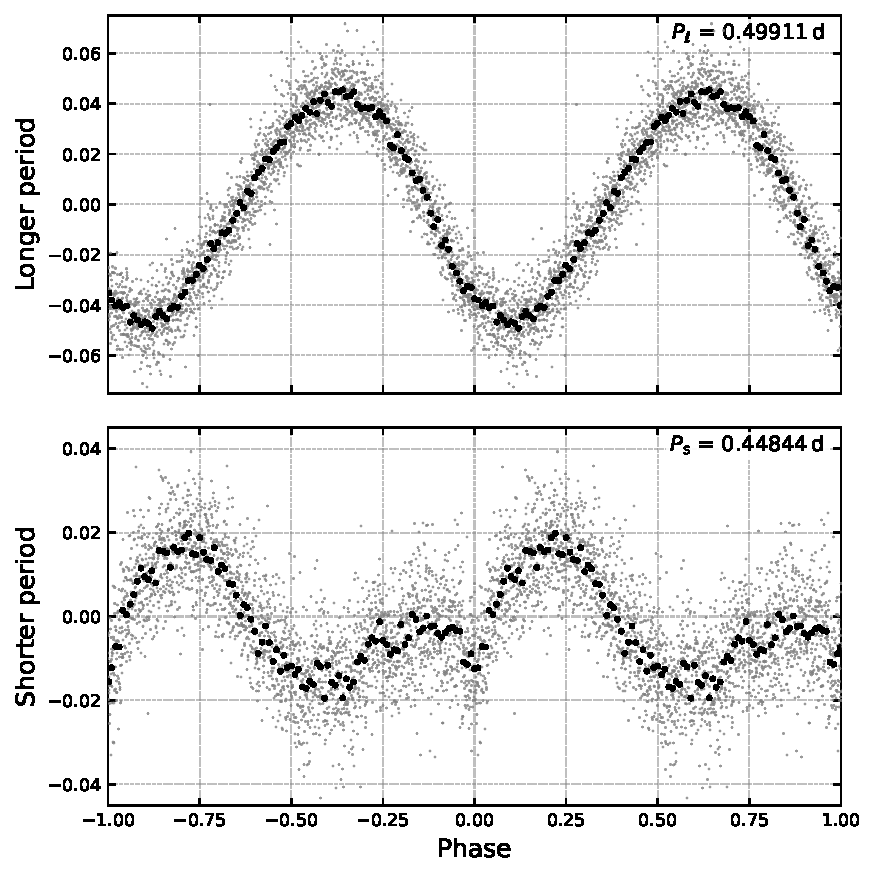
\includegraphics[width=0.48\textwidth]{f3.pdf}
	\end{center}
	\vspace{-0.7cm}
	\caption{ {\bf Scene used for blend analysis.}
		{\it Top:} Mean TESS image of PTFO 8-8695 over Sector~6, with a log-stretch.
		The position of PTFO 8-8695 is shown with a yellow star.
		Neighbors with $T<17$ are shown with orange crosses.
		The apertures used to measure the background and target star flux
		are shown with \texttt{X} and \texttt{/} hatches, respectively.
		{\it Bottom:} Digitized Sky Survey $R$-band image of the same field, with a linear stretch. The circles show
		apertures of radii 1, 1.5, and 2.25 pixels used in part of our blend
		analysis.
		The pixel level TESS data show that ``Star A''  does not contribute variability at either of the two observed periods (see Section~\ref{subsec:blend}).
		\label{fig:scene}
	}
\end{figure}

\begin{figure*}[t]
	\begin{center}
		\leavevmode
		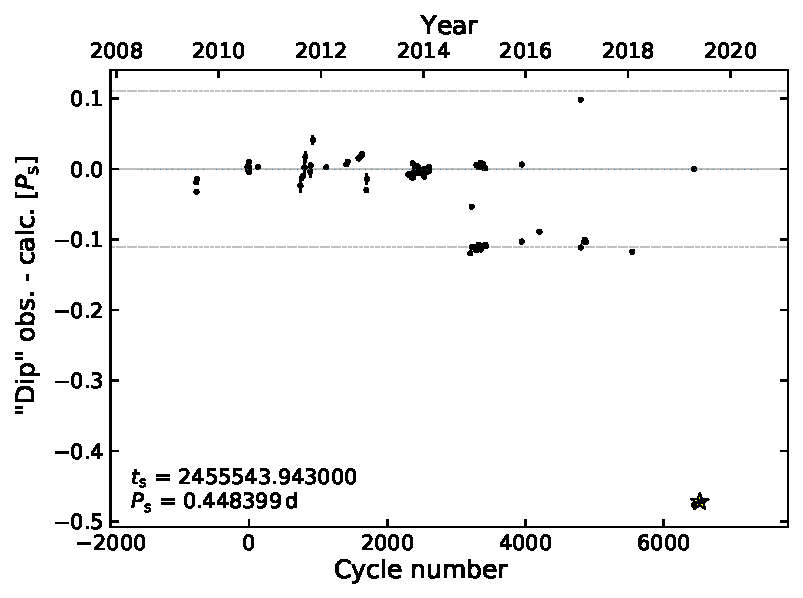
\includegraphics[width=0.9\textwidth]{f4.png}
	\end{center}
	\vspace{-0.7cm}
	\caption{ {\bf foo.}
		bar
		\label{fig:o_minus_c}
	}
\end{figure*}

\begin{figure*}[t]
	\begin{center}
		\leavevmode
		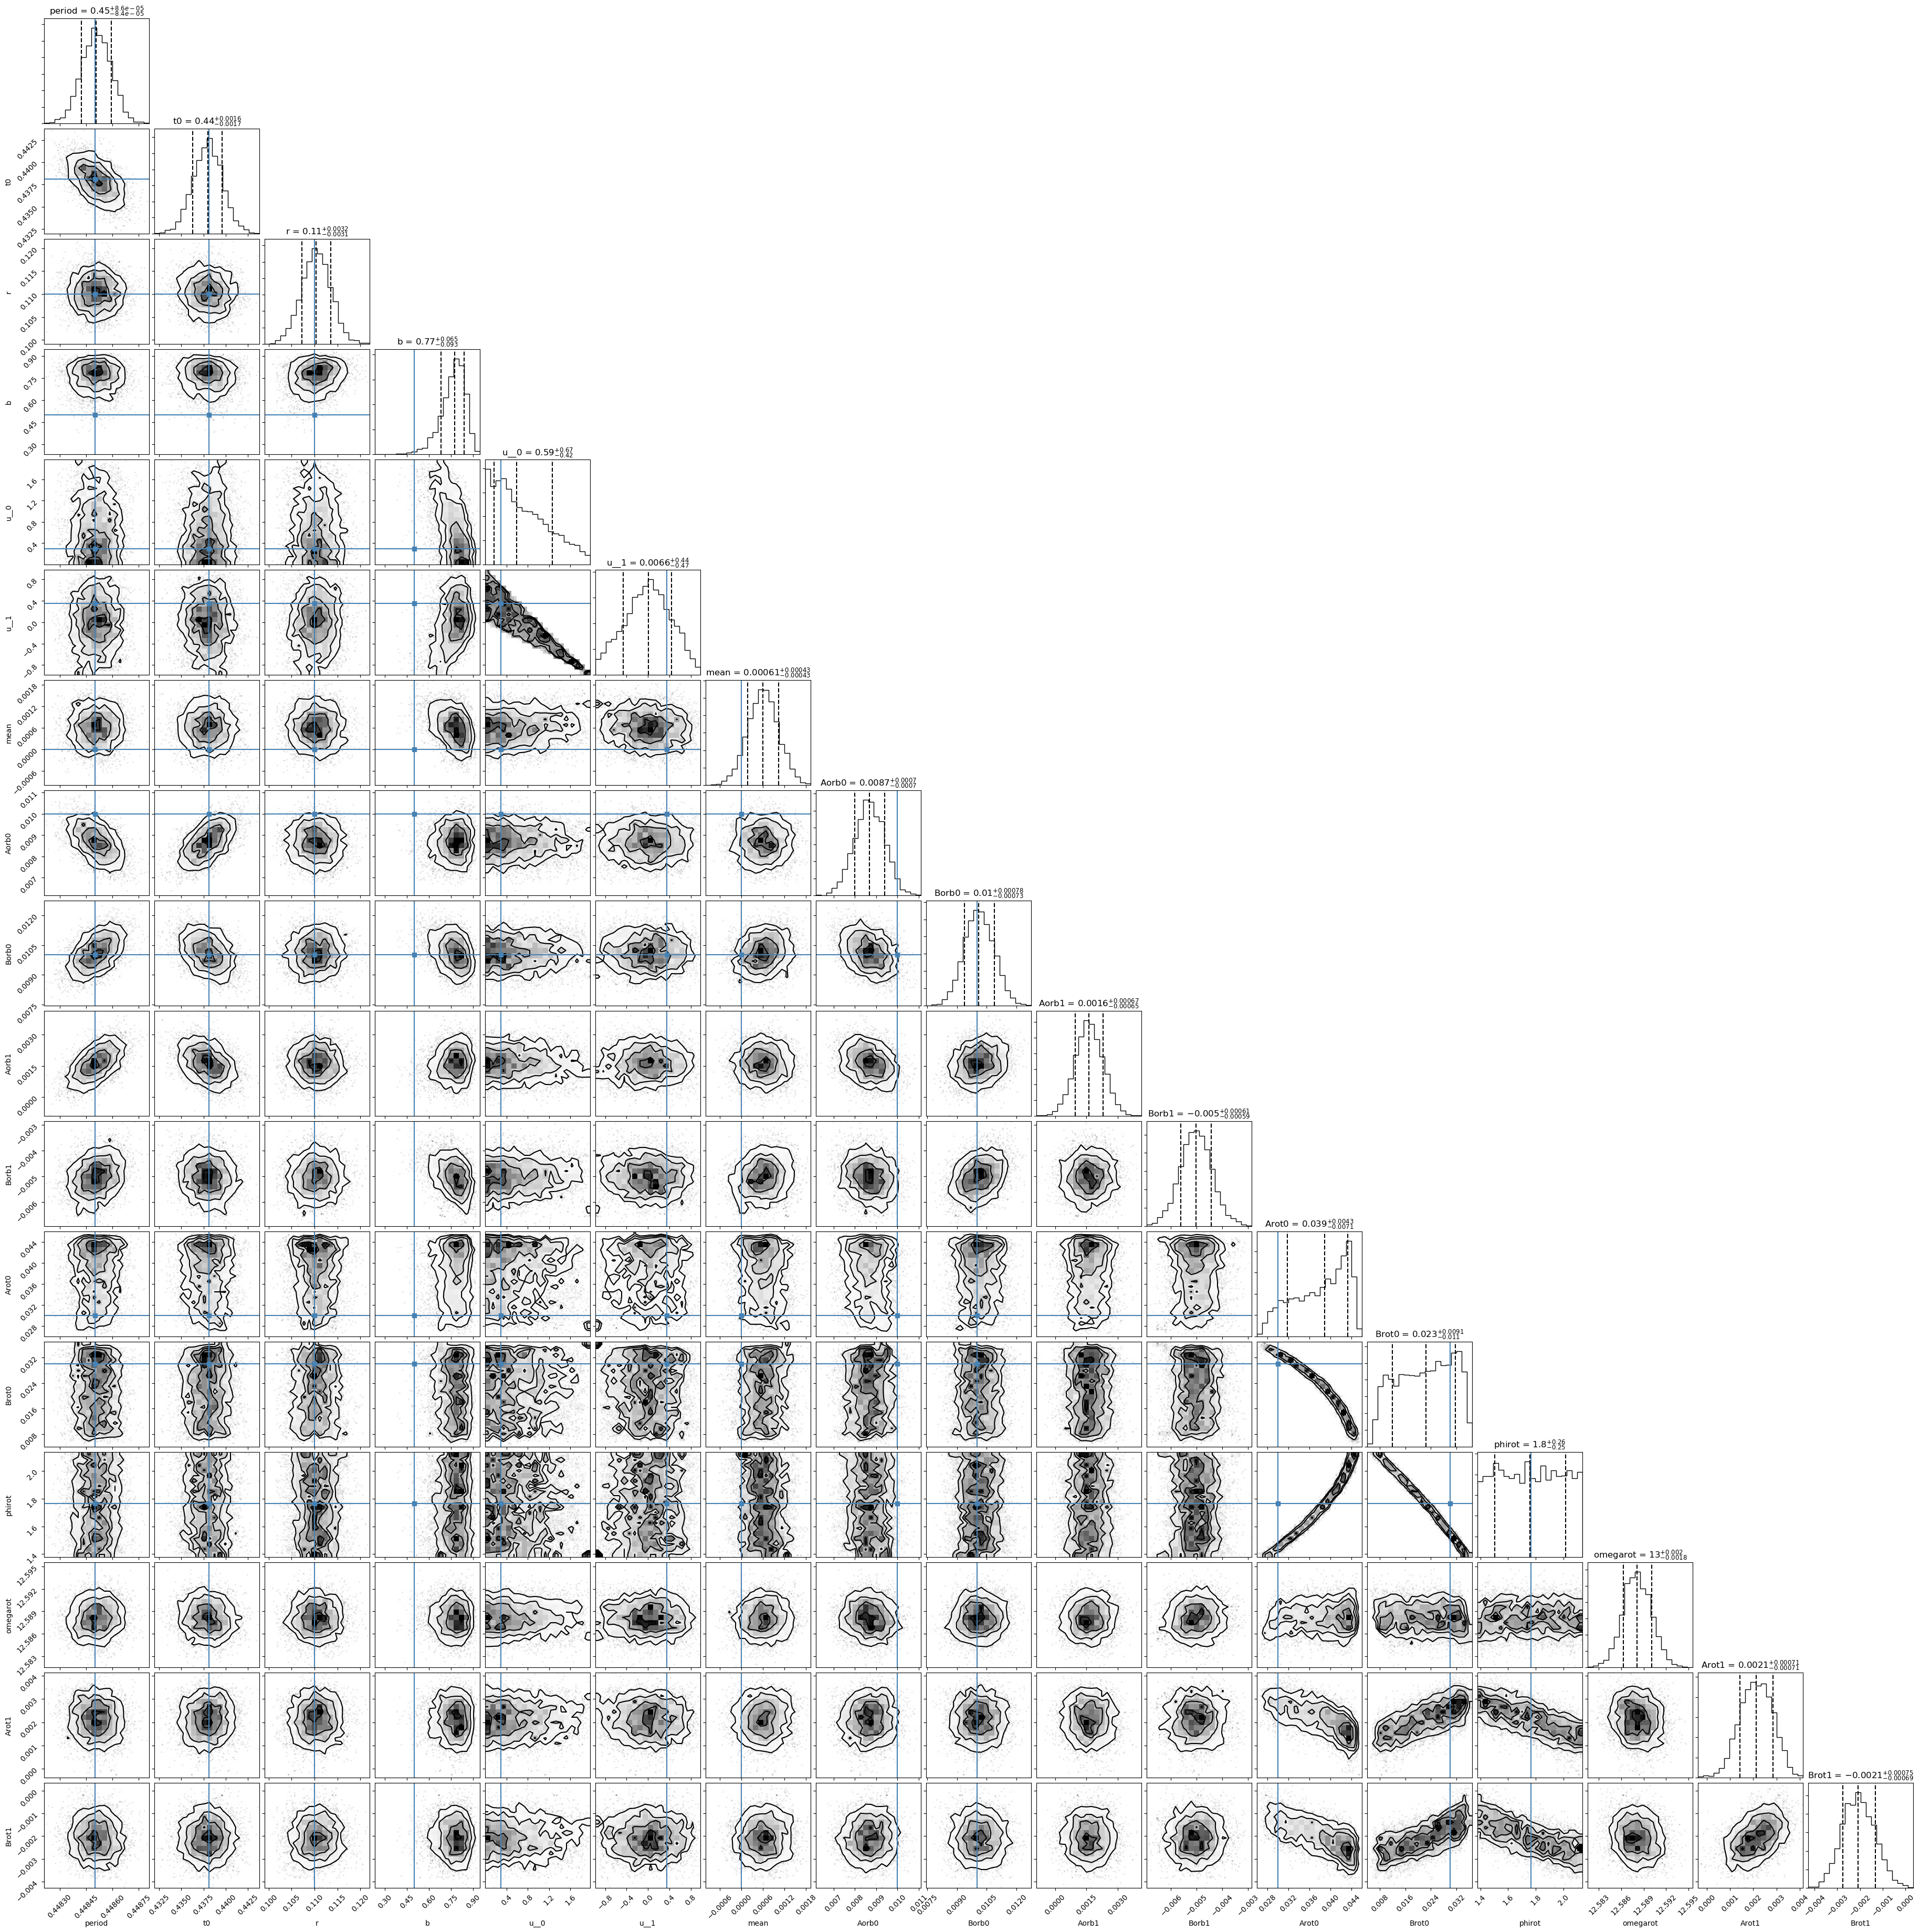
\includegraphics[width=0.9\textwidth]{f5_comp.png}
	\end{center}
	\vspace{-0.7cm}
	\caption{ {\bf foo.}
    bar
		\label{fig:corner}
	}
\end{figure*}


\subsection{Visual Inspection}

% TODO:
% Figure: CDIPS LC + SPOC LC (left two panels). Right panel:
% periodogram.
% 

\subsection{Model Fitting}

% I fitted some models of the form "transit + N harmonics of sines and
% cosines at the orbital frequency + M harmonics of sines and cosines at
% the rotation frequency". For example, if N=2 and M=1, then I fit for
% [logBrot0, logArot0, phirot, omegarot, logBorb1, logAorb1, logBorb0,
% logAorb0, b, r, u, logP, t0, meanflux]. A_N is the amplitude of the
% Nth harmonic sine function A_N * sin(N(ωt+φ)), B_N of the cosine. I
% went with quadratic limb darkening.
% 
% On fake data, I got the right parameters provided I didn't turn up the
% noise too high.
% 
% I gave it a pass on the PTFO data, binning from 2->10 minute sampling
% to speed up the execution time. Results from two models are below.
% Case 1 is N=2,M=1. Case 2 is N=2,M=2. Both fits are fine, and I get
% decent convergence with a few minutes each. The rotation parameters
% (phase + amplitudes) are quite correlated, so I set a reasonably
% strong prior on the rotation phase.
% 
% The main result that both models agree on: the extra power at the
% orbital frequency seems to not be ellipsoidal. Both of these models
% prefer to put the power at 1x the orbital frequency, not 2x the
% orbital frequency! This gives both Aorb0 and Borb0 non-zero, while
% Aorb1 and Borb1 seem to be more consistent with zero.


\paragraph{Fourier analysis}
Figure~\ref{fig:splitsignal} could also be given in the frequency
domain, rather than the time domain.
The largest peaks in 
the Lomb-Scargle periodogram (CITE) of the raw light-curve are
at $P_\rm {s}$ and $P_{\rm \ell}$.
Both peaks of course have aliases.
The $P_\rm {\ell}$ peak has larger ampitude.
Subtracting out the long-period signal, the short-period signal
dominates the periodogram, and vice-versa.
The periodogram of the final residual (Figure~\ref{fig:splitsignal}
bottom row) shows a weakly significant, poorly resolved peak at
$\approx$8 days, consistent with the visual impression in the time
domain that there could be a weak long-period signal present.


\subsection{Blend considerations}
\label{subsec:blend}

The TESS pixels are $\approx21$'' per side, and so we need to consider
whether light from neighboring stars could affect the photometry.  The
scene is shown in Figure~\ref{fig:scene}.  
The pixels used to
measure the background level are indicated with an `\texttt{X}' hatch,
and the pixels used for the final light-curve are shown with the
`\texttt{/}' hatch.

The target star, PTFO
8-8605 (TIC 264461976), has a $T$-band magnitude of 14.0, and its position is shown with a
star.  
The other (unlabeled) star inside the target aperture, TIC 264461979, has $T=16.8$ and so cannot
contribute a signal with relative amplitude 10\%.
The only neighbor that is sufficiently close and bright that
its light might contaminate the target star is TIC 264461980, with
$T=14.8$, which we denote ``Star A''.  Star A is 23.6'' NW of our
target, and based on the magnitude difference could contribute up to
48\% the flux of our target star, PTFO 8-8695.  

Because PTFO 8-8695 has previously been identified to have periodicity
consistent with our measurement of $P_{\rm s}$, our main concern
regarding blending is the degree to which we can be certain that the
long-period signal at $P_{\rm \ell}$ also originates from PTFO 8-8695.
We took two approaches towards determining the source of the long-period signal.

First, we examined the CDIPS full frame image light-curves of the
target, which are available on MAST \citep{bouma_cluster_2019}.
The maximal peak-to-peak beat amplitude is consistently $\approx$10\%
across apertures of radii 1, 1.5, and 2.25 pixels.
If Star A were the source of the long-period variability, we would expect the
peak variability amplitude to be smallest in the 1 pixel aperture, based on the
separation of the sources (Figure~\ref{fig:scene}, bottom).
From this test alone, it seems unlikely that Star A is the source of
the long-period signal.

Second, we examined the light-curve of each pixel in the scene
individually.  We opted to use the
interactive tools implemented in
\texttt{lightkurve} \citep{lightkurve_2018}.  If Star A were the
source of the long-period variability, we would expect the pixels
nearest to Star A to show a sinusoidal signal with
amplitude exceeding $10\%$.  We find no evidence for
this being the case.  The pixel directly below Star A does not
clearly show the sinusoidal variability, and the peak-to-peak 
variability in that pixel is $\lesssim 8\%$.  In contrast, the
south-easternmost pixel within PTFO 8-8695's aperture (the pixel 
furthest from Star A that was used in the optimal aperture) shows the $P_{\rm \ell}$ sinusoidal
variability signal at $\approx 10\%$ amplitude.

As there is no evidence in favor of a blend scenario, we
conclude that both the $P_{\rm s}$ and $P_{\rm \ell}$ signals originate from PTFO 8-8695.

\section{Discussion}
\label{sec:discussion}

The TESS dip does not phase up where it is supposed to...
\label{fig:o_minus_c}

\section{Conclusions}
\label{sec:conclusions}



%%%%%%%%%%%%%%%%%%%%%%%%%%%%%%%%%%%%%%%%%%%%%%%%%%%%%%%%%%%%%%%%%%%%%%%%%%%%%%%

% \acknowledgements
% %
% This paper includes data collected by the TESS mission, which are
% publicly available from the Mikulski Archive for Space Telescopes
% (MAST).
% %
% Funding for the TESS mission is provided by NASA's Science Mission
% directorate.
% %
% This work made use of NASA's Astrophysics Data System Bibliographic
% Services.
% %
% Based on observations obtained at the Gemini Observatory, which is
% operated by the Association of Universities for Research in Astronomy,
% Inc., under a cooperative agreement with the NSF on behalf of the
% Gemini partnership: the National Science Foundation (United States),
% National Research Council (Canada), CONICYT (Chile), Ministerio de
% Ciencia, Tecnolog\'{i}a e Innovaci\'{o}n Productiva (Argentina),
% Minist\'{e}rio da Ci\^{e}ncia, Tecnologia e Inova\c{c}\~{a}o (Brazil),
% and Korea Astronomy and Space Science Institute (Republic of Korea).
% %
% Observations in the paper made use of the High-Resolution Imaging
% instrument Zorro at Gemini-South. Zorro was funded by the NASA
% Exoplanet Exploration Program and built at the NASA Ames Research
% Center by Steve B. Howell, Nic Scott, Elliott P. Horch, and Emmett
% Quigley.
% %
% This research has made use of the VizieR catalogue access tool, CDS,
% Strasbourg, France. The original description of the VizieR service was
% published in A\&AS 143, 23.
% %
% This work has made use of data from the European Space Agency (ESA)
% mission {\it Gaia} (\url{https://www.cosmos.esa.int/gaia}), processed
% by the {\it Gaia} Data Processing and Analysis Consortium (DPAC,
% \url{https://www.cosmos.esa.int/web/gaia/dpac/consortium}). Funding
% for the DPAC has been provided by national institutions, in particular
% the institutions participating in the {\it Gaia} Multilateral
% Agreement.
%
% (Some of) The data presented herein were obtained at the W. M. Keck
% Observatory, which is operated as a scientific partnership among the
% California Institute of Technology, the University of California and
% the National Aeronautics and Space Administration. The Observatory was
% made possible by the generous financial support of the W. M. Keck
% Foundation.
% The authors wish to recognize and acknowledge the very significant
% cultural role and reverence that the summit of Maunakea has always had
% within the indigenous Hawaiian community.  We are most fortunate to
% have the opportunity to conduct observations from this mountain.
%
% \newline
%

\software{
  \texttt{astrobase} \citep{bhatti_astrobase_2018},
  % \texttt{astroplan} \citep{astroplan2018},
  \texttt{astropy} \citep{astropy_2018},
  \texttt{astroquery} \citep{astroquery_2018},
  % \texttt{BATMAN} \citep{kreidberg_batman_2015},
  \texttt{corner} \citep{corner_2016},
  \texttt{emcee} \citep{foreman-mackey_emcee_2013},
  \texttt{IPython} \citep{perez_2007},
	\texttt{lightkurve} \citep{lightkurve_2018},
  \texttt{matplotlib} \citep{hunter_matplotlib_2007}, 
  \texttt{MESA} \citep{paxton_modules_2011,paxton_modules_2013,paxton_modules_2015}
  \texttt{numpy} \citep{walt_numpy_2011}, 
  \texttt{pandas} \citep{mckinney-proc-scipy-2010},
  \texttt{radvel} \citep{fulton_radvel_2018},
  % \texttt{scikit-learn} \citep{scikit-learn},
  \texttt{scipy} \citep{jones_scipy_2001}.
}


% \facilities{
% 	{\it Astrometry}:
% 	Gaia \citep{gaia_collaboration_gaia_2016,gaia_collaboration_gaia_2018}.
% 	{\it Imaging}:
% 	Gemini:South~(Zorro; \citealt{scott_nessi_2018}.
% 	{\it Spectroscopy}:
% 	Keck:I~(HIRES; \citealt{vogt_hires_1994}),
% 	Euler1.2m~(CORALIE),
% 	ESO:3.6m~(HARPS; \citealt{mayor_setting_2003}).
% 	{\it Photometry}:
% 	CTIO:1.0m (Y4KCam),
% 	Danish 1.54m Telescope,
% 	El Sauce:0.356m,
% 	Elizabeth 1.0m at SAAO,
% 	Euler1.2m (EulerCam),
% 	Magellan:Baade (MagIC),
% 	Max Planck:2.2m	(GROND; \citealt{greiner_grond7-channel_2008})
% 	NTT,
% 	SOAR (SOI),
% 	TESS \citep{ricker_transiting_2015},
% 	TRAPPIST \citep{jehin_trappist_2011},
% 	VLT:Antu (FORS2).
% }

%
% The following are entries from Table 1 that are not otherwise cited
% in the text
%
% \nocite{wilson_wasp-4b_2008}
% \nocite{gillon_improved_2009}
% \nocite{winn_transit_2009}
% \nocite{hoyer_tramos_2013}
% \nocite{dragomir_terms_2011}
% \nocite{sanchis-ojeda_starspots_2011}
% \nocite{nikolov_wasp-4b_2012}
% \nocite{ranjan_atmospheric_2014}
% \nocite{huitson_gemini_2017}

% \input{WASP-4b_transit_time_table.tex}
% \input{WASP-4b_rv_table.tex}
% \input{model_fit_table.tex}
% \input{rv_model_posterior_table.tex}
% \input{pdot_table.tex}

%\clearpage
\bibliographystyle{yahapj}                            
\bibliography{bibliography} 


\listofchanges

\end{document}
